\chapter{Estudio de Diagramas de Fases}
\label{DF}





\section{Diagrama de Fases}
\begin{figure}
    \centering
    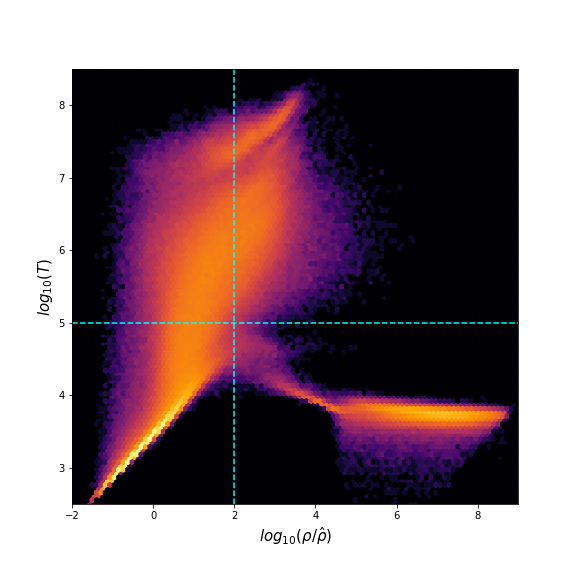
\includegraphics[width=14cm]{Figures/DF.png}
    \caption{Diagrama de Fase de la simulacion cosmologica. $\hat{\rho}$ es la desnidad media barionica del universo. NO HAY PROBLEMA CON LA FRACCION DE ESTRELLAS? Aca estoy alcanzando densidades de 8, que son altas (generalmente solo alcanzan hasta 6, ej paper que nos paso fede) pero debe ser por el modelo de SF, ya que aca da igual \citep{Springel2002}. KE ONDA. Poner etiqueta de las regiones}
    \label{DF}
\end{figure}{}

Las propiedades de los bariones pueden ser estudiadas observando los diagramas de fases, como el de la figura \ref{DF} donde las particulas de SPH se binean en el espacio de densidad y temperatura. Los procesos astrof\'isicos que ocurren a medida que el universo va evolucionando producen que las particulas de gas experimenten cambios en su densidad y temperatura. El colapso de los halos producen aumentos de densidad en el gas, feedback de supernovas producen aumento de la temperatura del gas, etc. 

Debido entonces a procesos astrof\'isicos, el gas va atravesando diferentes regiones del diagrama de fases, delimitadas por densidad y temperatura (linea punteada figura \ref{DF}. Estas regiones representan a particulas de gas que comparten ciertas propiedades f\'isicas en t\'erminos generales. Diversos autores utilizan diferentes criterios para clasificar de esta manera al gas (\cite{Schaal2016}, \cite{Martizzi2019}). En este trabajo se adopta el criterio utilizado por \citep{Huang2019} debido a que su simplicidad permite captar de manera general el comportamiento del gas. 

De esta manera entonces el gas se encuentra en el universo en 4 fases divididas por una temperatura  de  T=$10^{5}$K y una densidad $\delta_{th}$ definida por \citep{Kitayama1996} (( \citet{Dave2010} ACA ESTA BIEN, EN EL DE FEDE ESTA MAL LA FORMULA !!)) aquella en la que los halos se encuentran virilizados FIJATE BIEN ESTO:

\begin{equation}
    \delta_ {th}=6\pi^{2}(1+0.4093(1/f_{\Omega}-1)^{0.9052}-1
\end{equation}{}

\begin{equation}
    f_{\Omega}=\frac{\Omega_{m}(1+z)^{3}}{\Omega_{m}(1+z)^{3} + (1-\Omega_ {m} - \Omega_{\Lambda})(1+z)^{2} + \Omega_{\Lambda}}
\end{equation}{}
\begin{itemize}
    \item Gas difuso: Este gas es primordial, de baja densidad. La mayoria de este se encuentra en una curva que establece un balance entre enfriamiento adiab\'atico y calentamiento por fotoionizaci\'on. 
    \item WHIM: Las particulas de gas de esta regi\'on se encuentras ionizadas y a bajas densidades ya que son desplazadas aqu\'i debido a que en su proceso de colapso a los halos son calentadas por \textit{shocks} y frenan su caida a los halos.
    \item Condensado: Esta fase contiene gas frio que se encuentra dentro de los halos. 
    \item Caliente: Este gas se encuentra dentro de los halos, \textit{shocks} y \textit{feedbacks} debido a procesos astrof\'isicos elevan su temperatura. 
\end{itemize}{}
Cabe destacar que una quinta regi\'on se debe a el gas con formaci\'on estelar. Es gas dentro de los halos (condensado). Pero la resoluci\'on obtenida en nuestras simulaciones hace que en general las particulas pasen de estar Condensadas a convertirse en estrellas, sin permanecer mucho tiempo en la region de formaci\'on estelar. Es debido a esto que decidimos omitir esta regi\'on en el an\'alisis siguiente. 





\section{Perfiles del gas}

Tal como se sen\~alo con anterioridad, el gas en el universo se encuentra en diferentes \textit{fases} segun sus caracteristicas f\'isicas y sus propiedades f\'isicas van a depender de el entorno en el que se encuentren. De modo que las diferentes fases del gas trazan diferentemente las estructuras del universo, en particulas los perfiles de los vac\'ios cosmol\'ogicos. 

La tabla \ref{FraccionesGasTabla} contiene las fracciones $(f_{fase})$ de las fases en las que se encuentra el universo actual. Con esta informaci\'on es posible conocer la densidad media de cada fase $\hat{\rho}_{fase}$ que va a venir dada por:
\begin{equation}
    \hat{\rho}_{fase}=\rho_{crit}\Omega_{bar}f_{fase}
\end{equation}{}

Conociendo la densidad media de las fases es posible calcular el contraste de densidad siguiendo la ecuaci\'on \ref{ContrasteDensidad} y de esta manera podemos construir los perfiles de la figura \ref{PerfilGas}.


\begin{figure}
    \centering
    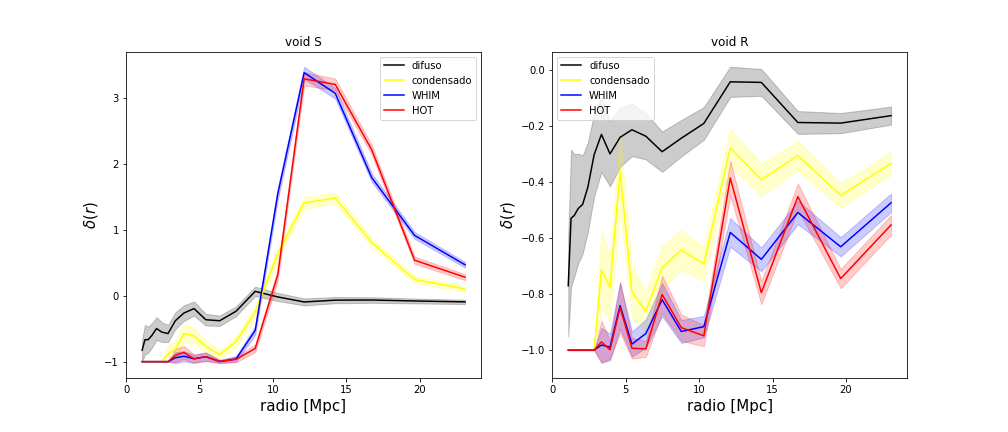
\includegraphics[width=14cm]{Figures/perfilgas.png}
    \caption{Caption}
    \label{PerfilGas}
\end{figure}{}

Es interesante observar que las diferentes fases del gas trazan la estructura de manera muy diferente. En el caso de el void S podemos ver como el gas \textit{Whim} y \textit{HOT} trazan la pared de el vac\'io de una manera muy pronunciada, mientras que el gas \textit{condensado} es sensible a la pared pero de forma menos intensa. El gas \textit{difuso} parece ser impermeable a la estructura ya que casi no presenta variaciones a lo largo del perfil, solo en el centro del void dentro de $\sim 5$ Mpc se observa un decrecimiento significativo de este perfil. 

El perfil de el void R presenta un crecimiento continuo desde el centro del vac\'io hacia el exterior. En el caso de el gas difuso el comportamiento parece ser similar a el void S ya que tenemos que crece fuertemente hasta $\sim 5$ Mpc pero luego parece estabilizarse, mas all\'a de un leve pico en el radio del void ($r\sim10$ Mpc. Las dem\'as fases de el gas trazan el perfil de una manera similar marcando un continu\'o crecimiento. 

Una diferencia importante parece ser marcada por el gas condensado y el gas caliente (en sus dos fases \textit{HOT} y \textit{WHIM}). Para el void S el gas condensado tiene un contraste menos intenso, mientras que para el void R el gas condensado tiene un contraste siempre mayor que el gas caliente. \textcolor{green}{Esto podr\'ia deberse a que el void S tiene una pared muy importante de gran densidad, donde se concentran los procesos de formaci\'on estelar, que mediante el feedback se encargan de calentar el gas y marcando de esta manera el contraste de densidad intenso que se observa para el gas en sus fases caliente.}

En la figura \ref{VoidFases} observamos un corte transversal que pasa por el centro del void S donde podemos ver donde se encuentra el gas de cada Fase. Podemos ver que el contraste es mas t\'enue en el gas difuso, que lo podemos encontrar tanto en las estructuras filamentosas que se observan como en la regi\'on interna que pertenece al centro del void. El gas \textit{condensado} y \textit{hot} se encuentra en regiones localizadas de los filamentos, en los halos. Esto es obvio ya que estamos hablando de gas a alta densidad que se encuentra colapsado en los halos de materia oscura. El gas \textit{WHIM} se encuentra como podemos ver en la estructura filamentosa que circunda al void. Esta gas es calentado en el proceso de colapso de los halos por lo cual es esperable que se halle entonces cerca de los mismos. 

\begin{figure}
    \centering
    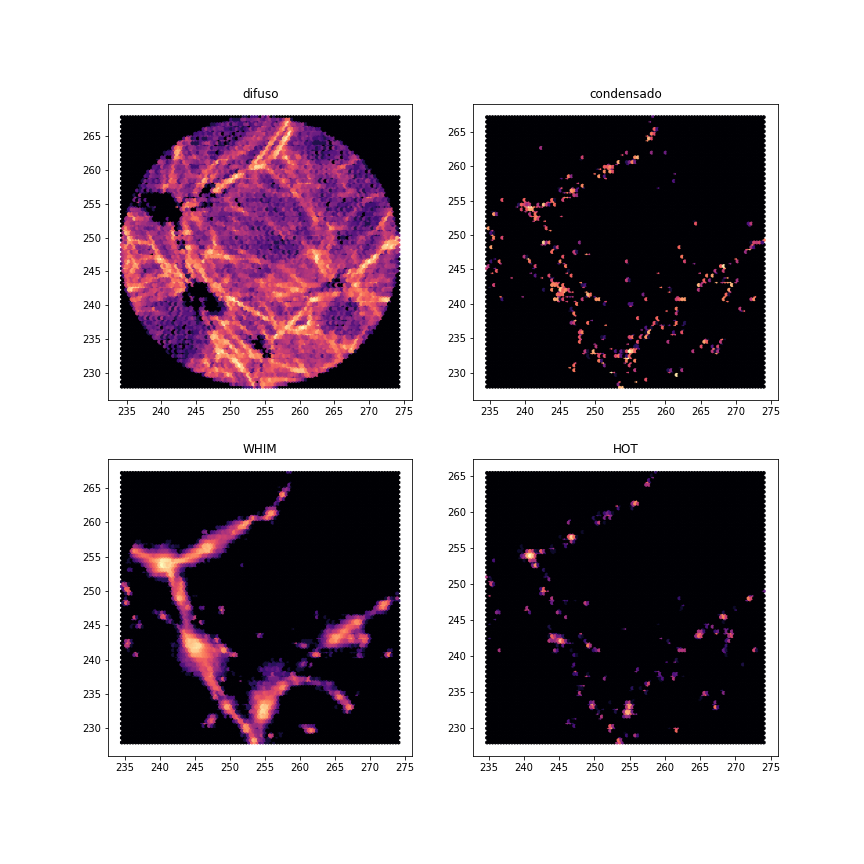
\includegraphics[width=14cm]{Figures/FasesHexbin_S.png}
    \caption{Caption}
    \label{VoidFases}
\end{figure}{}

\section{Universos pristinos}

Galaxias que habitan los voids tienen una historia de formaci\'on estelar y evoluci\'on qu\'mica de aquellas que habitan entornos de mas alta densidad. REF  (see e.g. Peebles 2001;Gottl ̈ober et al. 2003; Hoeft et al. 2006; Hahn et al. 2007a,b, andreferences therein).

Esto puede entenderse ya que los voids poseen un flujo de halos hacia las paredes de los mismos. (ACA MANDAR A EL PLOT DE EL PERF DE VELOCIDADES) por lo que la historia evolutiva de los halos y sus mergers va a ser diferente de aquellos halos que habiten entornos de mas alta densidad. En particular es esperable que la tasa de mergers de galaxias sea menor en los voids, de esta manera, las galaxias que habiten estos entornos ser\'an menos evolucionadas. 

Estas propiedades observadas de las galaxias que habitan los voids \citep{Kreckel2016} permiten pensar a los voids como universos pristinos, en el sentido de que las galaxias que habiten estos ambientes podr\'ian ser representativas de la poblaci\'on de galaxias de un universo temprano a alto redshift. 

Con motivo de explorar esta idea nos centramos en el estudio de los diagramas de fases, para evaluar en que medida las fracciones de bariones en cada fase del gas dentro de los voids puede compararse con las fracciones de bariones de el universo temprano. Es esperable que el universo temprano presente un mayor contenido de gas \textit{difuso} y menor contenido de gas dentro de los halos, ya sea en su fase de \textit{condensado} o \textit{caliente}. La figura \ref{TimeMachine} (central) presenta en diagrama de fases del universo a $z\sim3.2$ donde efectivamente podemos observar lo se\~nalado. La mayor parte del gas ocupa la region correspondiente a gas \textit{difuso} (un $\sim 85\%$) en comparaci\'on de al universo a z=0 donde el gas difuso ocupa un $\sim45\%$


\begin{table}[ht]
\begin{tabular}{c|c|c|c|c|c}
    - & void S & void R & universo $z\sim 3.2$ &universo $z\sim 2.7$ &universo z=0 \\
\hline    difuso     & 86.2  & 81.1  & 87.1  &  82.6   & 44.7\\
\hline    WHIM       & 1.6   & 4.2   & 2.2   &  4.2    & 24.8\\
\hline    caliente   & 2.3   & 4.5   & 1.1   &  2.3    & 16.8\\
\hline    condensado & 9.8   & 10.1  & 9.4   &  10.9   & 14.3\\
\hline
\end{tabular}
\caption{..}
\label{FraccionesGasTabla}
\end{table}

De modo que puede realizarse una comparaci\'on \textit{gruesa} estudiando fracciones de bariones dentro del void a z=0 con una regi\'on homogenea del universo a diferentes redshifts para ver donde son mas similares las fracciones de gas. Para lo cual se utilizo la simulacion BASE ?? Externo al vOIDS?? 

Para seleccionar las particulas pertenecientes al void, se busco que el contraste adimencional de densidad integrado de la masa sea $\Delta(r)_{masa}<-0.6$. Esto se corresponde a los radios $r_{S}=8.1Mpc$ y $r_{R}=8.8 Mpc$ para los diferentes voids. Con las particulas seleccionadas dentro de estos radios se contruyeron los diagramas de fase de la figura \ref{TimeMachine} (izquierda y derecha). 


La figura \ref{Error} representa el error cuadr\'atico (\ref{ErrorFormula}) de las fracciones de gas del void-universo a diferentes edades. Podemos observar que el universo a $z\sim2.9$ se asemeja al void R, mientras que a $z\sim3.5$ el se asemeja al void S, en este \'ultimo caso, las similitudes son mayores. 


\begin{equation}
    \epsilon=\sum_{i=fases}(f^{void}_{i}-f^{univ}_{i})^{2}
    \label{ErrorFormula}
\end{equation}{}


Una primera vista a la figura \ref{TimeMachine} permite apreciar la similitud de los diagramas de fases. Practicamente observamos una carencia de particulas calientes a diferencia de el diagrama \ref{DF}. Esto se debe, en el caso del universo a z$\sim$3 a que los halos no han terminado de colapsarse y los que hay son peque\~nos. Esto produce que no hayan formado una cantidad suficiente de estrellas como para calentar el entorno. En el caso de los voids, al ser ambientes subdensos el proceso de formaci\'on de los halos se retrasa respecto a el universo en general. De esta manera es que se traza una similitud entre los voids y su similitud con el universo pristino. 

\textbf{Llama la atenci\'on que nuestra epoca de myor similitud coincide con la epoca de mayor formaci\'on estelear de nuestras simulaciones.}





\begin{figure}
    \centering
    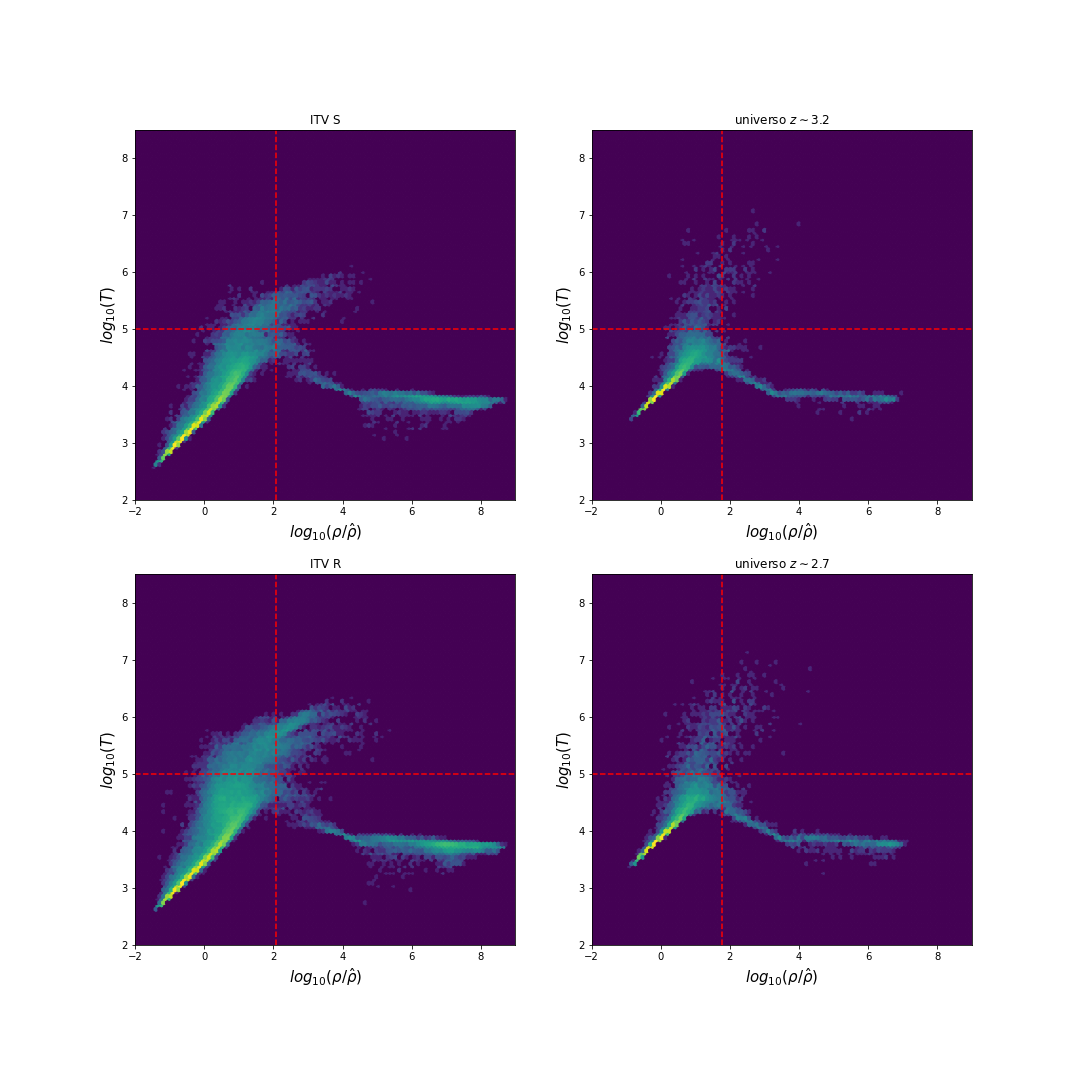
\includegraphics[width=14cm]{Figures/TimeMachine_DF.png}
    \caption{Caption}
    \label{TimeMachine}
\end{figure}{}

\begin{figure}
    \centering
    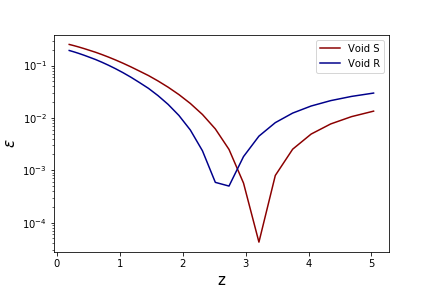
\includegraphics[width=12cm]{Figures/TimeMachine_error.png}
    \caption{Error cuadratico de las fracciones de gas del universo en comparaci\'on a los voids. }
    \label{Error}
\end{figure}{}

Como puede apreciarse en la figura \ref{TimeMachine} el gas difuso parece comportarse como una relaci\'on de potencia entre la densidad y la temperatura. Esto fue estudiado por \citep{Hui1997} donde se demostro que existe una relaci\'on de tal naturaleza que modela los procesos de contracci\'on adiab\'atica y calentamiento por fotoionizaci\'on. 
\begin{equation}
    T=T_{0}(1+\delta)^{\gamma-1}
    \label{EcuacionEstado}
\end{equation}{}
La relaci\'on \ref{EcuacionEstado} modela entonces el comportamiento del gas poco denso del IGM. 





